\section{BAM}
Progetto sviluppato in collaborazione con il CNG

\label{sec:chapter_4_section_1}
\subsection*{Appendiabiti}
\begin{figure}[htbp] %  figure placement: here, top, bottom, or page
   \centering
   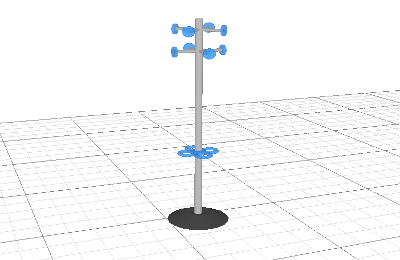
\includegraphics[width=0.5\linewidth]{images/hanger}
   \caption{Modello 3D appendiabiti}
   \label{fig:appendiabiti}
\end{figure}
(see Figure~\ref{fig:appendiabiti})
\newpage

\subsection*{Armadietto}
\begin{figure}[htbp] %  figure placement: here, top, bottom, or page
   \centering
   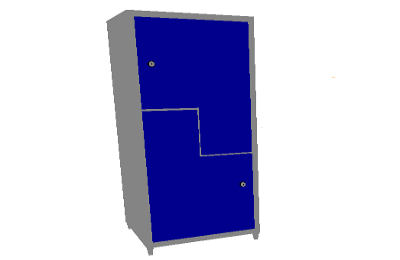
\includegraphics[width=0.5\linewidth]{images/wardrobe}
   \caption{Modello 3D armadietto}
   \label{fig:armadietto}
   \end{figure}
   (see Figure~\ref{fig:armadietto})
\newpage

\subsection*{Attaccapanni}
\begin{figure}[htbp] %  figure placement: here, top, bottom, or page
   \centering
   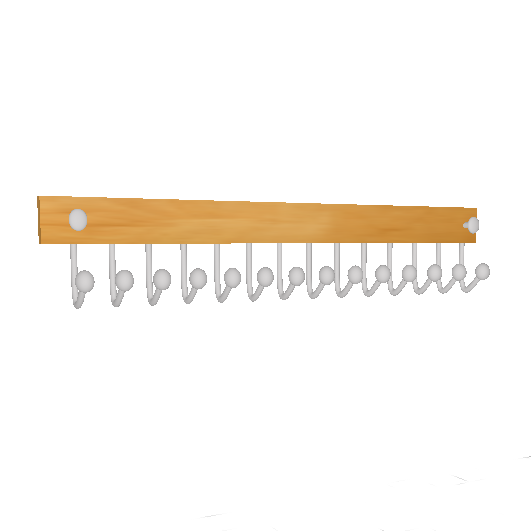
\includegraphics[width=0.5\linewidth]{images/attaccapanni2}
   \caption{Modello 3D attaccapanni}
   \label{fig:attaccapanni}
   \end{figure}
   (see Figure~\ref{fig:attaccapanni})
   \newpage

\subsection*{Banco}
\begin{figure}[htbp] %  figure placement: here, top, bottom, or page
   \centering
   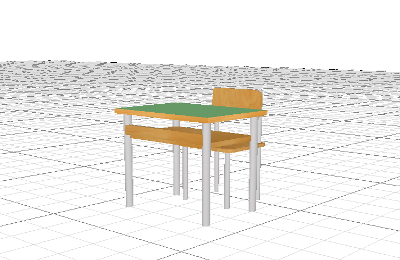
\includegraphics[width=0.5\linewidth]{images/banco2}
   \caption{Modello 3D banco}
   \label{fig:banco}
   \end{figure}
   (see Figure~\ref{fig:banco})
   \newpage

\subsection*{Cattedra}
\begin{figure}[htbp] %  figure placement: here, top, bottom, or page
   \centering
   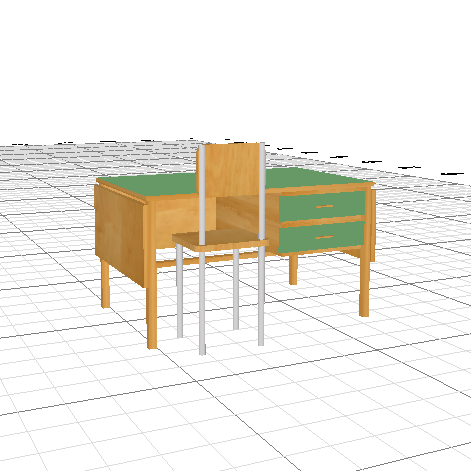
\includegraphics[width=0.5\linewidth]{images/cattedra2}
   \caption{Modello 3D cattedra}
   \label{fig:cattedra}
   \end{figure}
   (see Figure~\ref{fig:cattedra})
   \newpage

\subsection*{Cestino}
\begin{figure}[htbp] %  figure placement: here, top, bottom, or page
   \centering
   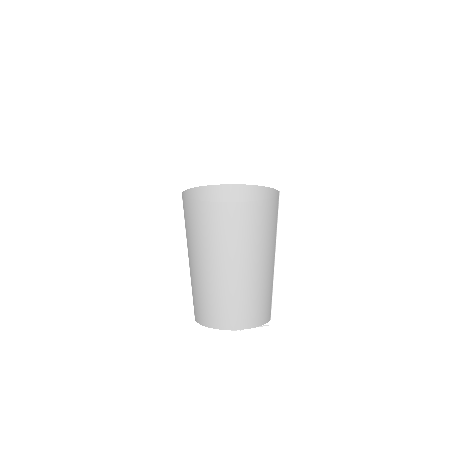
\includegraphics[width=0.5\linewidth]{images/cestino}
   \caption{Modello 3D cestino}
   \label{fig:cestino}
   \end{figure}
   (see Figure~\ref{fig:cestino})
   \newpage

\subsection*{Condizionatore}
\begin{figure}[htbp] %  figure placement: here, top, bottom, or page
   \centering
   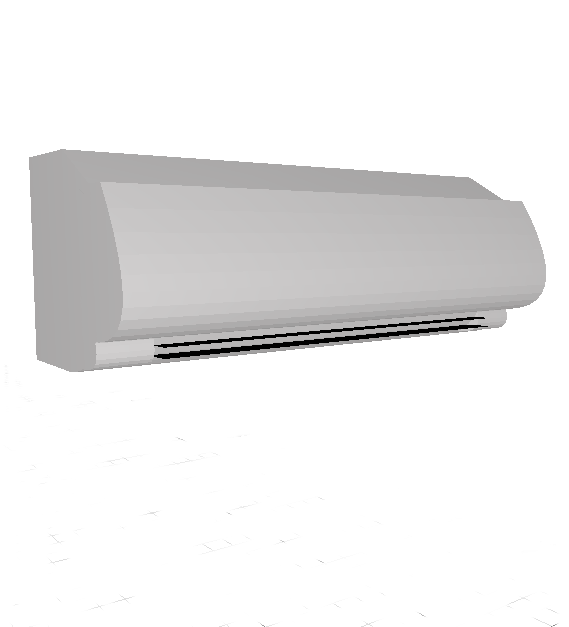
\includegraphics[width=0.5\linewidth]{images/condizionatore}
   \caption{Modello 3D condizionatore}
   \label{fig:condizionatore}
   \end{figure}
   (see Figure~\ref{fig:condizionatore})
   \newpage

\subsection*{Lavagna}
\begin{figure}[htbp] %  figure placement: here, top, bottom, or page
   \centering
   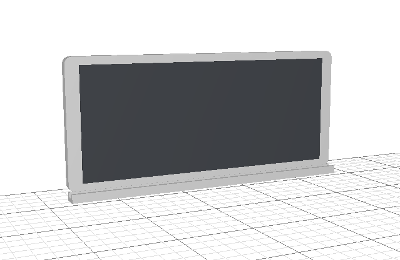
\includegraphics[width=0.5\linewidth]{images/lavagna}
   \caption{Modello 3D lavagna}
   \label{fig:lavagna}
   \end{figure}
   (see Figure~\ref{fig:lavagna})
   \newpage

\subsection*{Libreria}
\begin{figure}[htbp] %  figure placement: here, top, bottom, or page
   \centering
   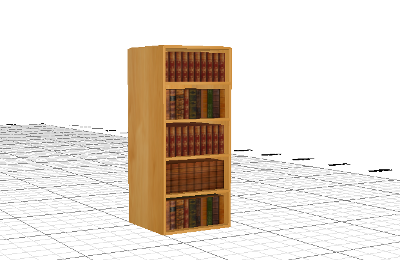
\includegraphics[width=0.5\linewidth]{images/bookcase}
   \caption{Modello 3D libreria}
   \label{fig:libreria}
   \end{figure}
   (see Figure~\ref{fig:libreria})
   \newpage

\subsection*{Lim}
\begin{figure}[htbp] %  figure placement: here, top, bottom, or page
   \centering
   
\includegraphics[width=0.5\linewidth]{images/lim}
   \caption{Modello 3D lim}
   \label{fig:lim}
   \end{figure}
   (see Figure~\ref{fig:lim})
   \newpage

\subsection*{Porta Ombrelli}
\begin{figure}[htbp] %  figure placement: here, top, bottom, or page
   \centering
   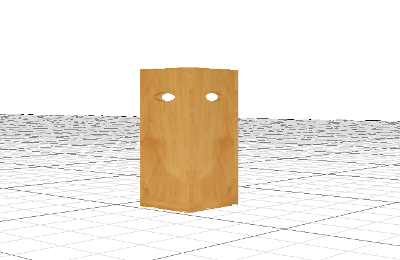
\includegraphics[width=0.5\linewidth]{images/portaombrelli}
   \caption{Modello 3D porta ombrelli}
   \label{fig:portaombrelli}
   \end{figure}
   (see Figure~\ref{fig:portaombrelli})
   \newpage

\subsection*{Cestini Differenziata}
\begin{figure}[htbp] %  figure placement: here, top, bottom, or page
   \centering
   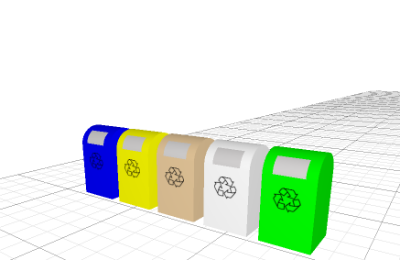
\includegraphics[width=0.5\linewidth]{images/recycling-bins}
   \caption{Modello 3D cestini differenziata}
   \label{fig:differenziata}
   \end{figure}
   (see Figure~\ref{fig:differenziata})
   \newpage

\subsection*{Termosifone}
\begin{figure}[htbp] %  figure placement: here, top, bottom, or page
   \centering
   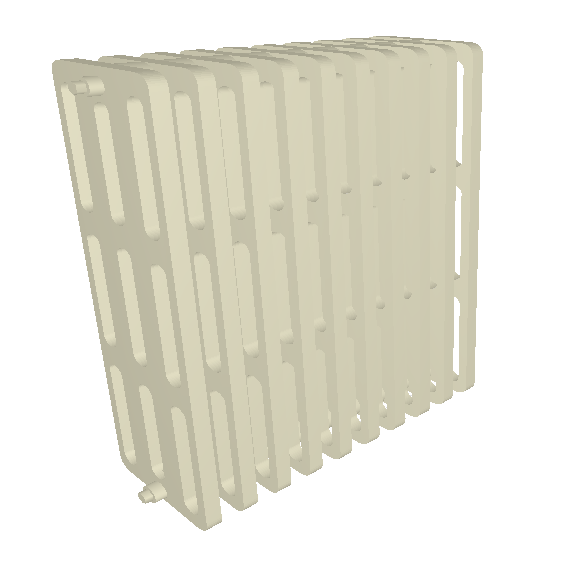
\includegraphics[width=0.5\linewidth]{images/termosifone}
   \caption{Modello 3D termosifone}
   \label{fig:termosifone}
   \end{figure}
   (see Figure~\ref{fig:termosifone})
   \newpage

\subsection*{Finestra con Veneziana}
\begin{figure}[htbp] %  figure placement: here, top, bottom, or page
   \centering
   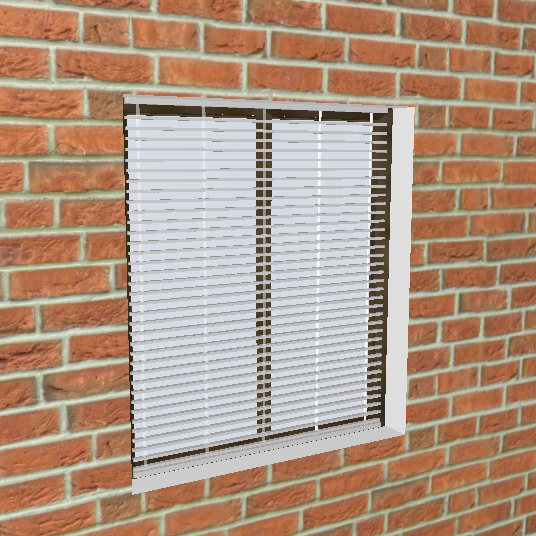
\includegraphics[width=0.5\linewidth]{images/veneziana}
   \caption{Modello 3D finestra con veneziana}
   \label{fig:veneziana}
   \end{figure}
   (see Figure~\ref{fig:veneziana})
   \newpage

\subsection*{Finestra con Tenda}
\begin{figure}[htbp] %  figure placement: here, top, bottom, or page
   \centering
   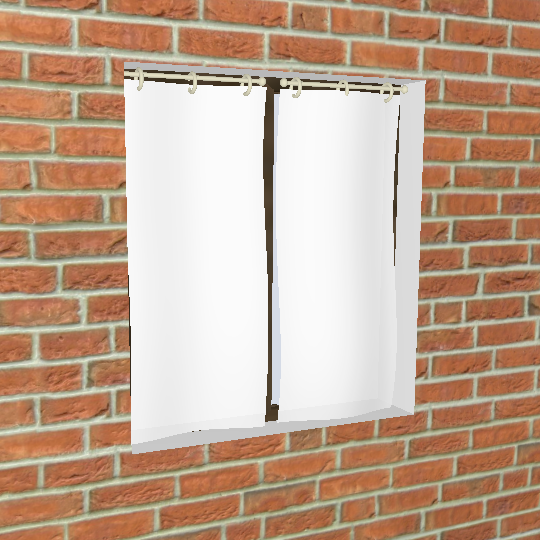
\includegraphics[width=0.5\linewidth]{images/tenda}
   \caption{Modello 3D finestra con tenda}
   \label{fig:tenda}
   \end{figure}
   (see Figure~\ref{fig:tenda})
   \newpage
